\thispagestyle{plain}

\chapter{Marco Teórico}
	\section{Normas de Calidad}
			ISO (Organización Internacional de Normalización) es una federación mundial de organismos
			nacionales de normalización (organismos miembros de ISO). El trabajo de preparación de las normas
			internacionales normalmente se realiza a través de los comités técnicos de ISO. Cada organismo
			miembro interesado en una materia para la cual se haya establecido un comité técnico, tiene el derecho
			de estar representado en dicho comité. Las organizaciones internacionales, públicas y privadas, en
			coordinación con ISO, también participan en el trabajo. ISO colabora estrechamente con la Comisión
			Electrotécnica Internacional (IEC) en todas las materias de normalización electrotécnica.
		\subsection{ISO 9000:2015}
			\subsubsection{Generalidades}
				\par
					Los conceptos y los principios de la gestión de la calidad descritos en esta Norma Internacional
					proporcionan a la organización la capacidad de cumplir los retos presentados por un entorno que es
					profundamente diferente al de décadas recientes El contexto en el que trabaja una organización
					actualmente se caracteriza por el cambio acelerado, la globalización de los mercados, los recursos
					limitados y la aparición del conocimiento como un recurso principal El impacto de la calidad se extiende
					más allá de la satisfacción del cliente puede tener además un impacto directo en la reputación de la
					organización.
					
				\newpage
				\thispagestyle{plain}
				
				\par 
					\noindent La sociedad está más formada y demanda más. lo que hace a las parles interesadas más influyentes
					progresivamente. Esta Norma Internacional proporciona una manera de pensar más amplia en relación
					con la organización, proporcionando conceptos y principios fundamentales para utilizar en el desarrollo
					de un Sistema de Gestión de la Calidad (SGC).
					
				\par \noindent 
					Todos los conceptos, principios y sus interrelaciones deberían verse como un conjunto y no aislados unos de otros. Un concepto o principio individual no es más importante que otro. En cada momento es crítico encontrar un balance correcto en su aplicación.
						
			\subsubsection{Conceptos Fundamentales}
				
				\paragraph{Calidad}
					Una organización orientada la calidad promueva una cultura que da como resultado comportamientos,
					actitudes, actividades y procesos para proporcionar valor mediante el cumplimiento de las necesidades y
					expectativas de los clientes y otras partes interesadas pertinentes.
					
					\par 
						\noindent La calidad de los productos y servicios de una organización está determinada por la capacidad para
						satisfacer a los clientes, y por el impacto previsto y el no previsto sobre las partes interesadas
						pertinentes.
						
					\par 
						\noindent La calidad de los productos y servicios incluye no solo su función y desempeño previstos, sino también su valor percibido y el beneficio para el cliente.
					
				\paragraph{Sistemas de gestión de calidad}
					Un SGC comprende actividades mediante las que la organización identifica sus objetivos y determina los
					procesos y recursos requeridos para lograr los resultados deseados.
					El SGC gestiona los procesos que interactúan y los recursos que se requieren para proporcionar valor y
					lograr los resultados para las partes interesadas pertinentes.
					
					\par 
						\noindent EL SGC posibilita a la alta dirección optimizar el uso de los recursos considerando las consecuencias de sus decisiones a largo y corto plazo.
						
				\paragraph{Contexto de una organización}
					Comprender el contexto de una organización es un proceso Este proceso determina los factores que
					influyen en el propósito, objetivos y sostenibilidad de la organización. Considera factores internos tales
					como los valores, cultura, conocimiento y desempeño de la organización. También considera factores
					externos tales como entornos legales, tecnológicos, de competitividad. de mercados, culturales, sociales
					y económicos.
					
					\newpage
					\thispagestyle{plain}
					
					\par	
						\noindent La visión, misión, políticas y objetivos son ejemplos de las formas en las pueden expresar los propósitos
						de la organización.
						
					\paragraph{Partes interesadas}
						El concepto de partes interesadas se extiende más allá del enfoque únicamente al cliente. Es importante
						considerar todas las partes interesadas pertinentes.
						
					\par 
						\noindent Parte del proceso para la comprensión del contexto de la organización es identificar sus partes
						interesadas. Las partes interesadas pertinentes son aquellas que generan riesgo significativo para la
						sostenibilidad de la organización si sus necesidades y expectativas no se cumplen. Las organizaciones
						definen qué resultados son necesarios para proporcionar a aquellas partes interesadas pertinentes para
						reducir dicho riesgo
						
					\par 
						\noindent Las organizaciones atraen, consiguen y conservan el apoyo de las partes interesadas pertinentes de las
						que dependen para su éxito
							
				\subsubsection{Principios de la gestión de la calidad}
					\paragraph{Enfoque al cliente}
						El enfoque principal dela gestión de la calidad es cumplir con los requisitos del cliente y tratar de exceder
						las expectativas del cliente.
					\paragraph{Liderazgo}
						Los líderes en todos los niveles establecen la unidad de propósito y la dirección y crean condiciones en
						las que las personas se implican en el logro de los objetivos de la calidad de la organización.
					\paragraph{Compromiso de las personas}
						Las personas competentes, empoderadas y comprometidas en toda la organización son esenciales para
						aumentar la capacidad de la organización para generar y proporcionar valor.
					\paragraph{Enfoque a procesos}
						Se alcanzan resultados coherentes y previsibles de manera mas eficaz y eficiente cuando las actividades
						se entienden y gestionan como procesos interrelacionados que funcionan como un sistema coherente.
					\paragraph{Mejora}
						Las organizaciones con éxito tienen un enfoque continuo hacia la mejora.
						
					\newpage
					\thispagestyle{plain}
					
					\paragraph{Toma de decisiones basada en evidencia}
						Las decisiones basadas en el análisis y la evaluación de datos e información tienen mayor probabilidad
						de producir los resultados deseados.
					
					\paragraph{Gestión de relaciones}
						Para el éxito sostenido, las organizaciones gestionan sus relaciones con las partes interesadas
						pertinentes, tales como los proveedores.
				
				\subsubsection{Términos y definiciones}
					\paragraph{Términos relativos a la persona o personas}
						\begin{itemize}
							\item Alta Dirección: Persona o grupo de personas que dirige y controla una organización al más alto nivel.
							
							\item Participación Activa: Tomar parte en una actividad, evento o situación.
							
							\item Compromiso: Participación Activa en, y contribución a, las actividades para lograr objetivos compartidos
						\end{itemize}
					
					\paragraph{Términos relativos a la organización}
						\begin{itemize}
							\item Organización: Persona o grupo de personas que tiene sus propias funciones con responsabilidades, autoridades y
							relaciones para lograr sus objetivos.
							
							\item Contexto de la organización: Combinación de cuestiones internas y externas que pueden tener un efecto en el enfoque de la
							organización para el desarrollo y logro de sus objetivos.
							
							\item Parte interesada: Persona u organización que puede afectar, verse afectada o percibirse como afectada por una
							decisión o actividad.
							
							\item Cliente: Persona u organización  que podría recibir o que recibe un producto o un servicio
							destinado a esa persona u organización o requerido por ella.
							
							\item Proveedor: Organización que proporciona un producto o un servicio
							
							\item Proveedor externo: Proveedor que no es parte de la organización.
							
							\item Proveedor de PRC: (Proveedor de un proceso de resolución de conflictos)
							Persona u organización que provee y opera un proceso de resolución de conflictos externo.
							
							\newpage
							\thispagestyle{plain}
							
							\item Asociación:  organización formada por organizaciones o personas miembro. 
							
							\item Función metrológica: Unidad funcional con responsabilidad administrativa y técnica para definir e implementar el sistema de
							gestión de las mediciones.
							
						\end{itemize}
					
					\paragraph{Términos relativos a la actividad}
						\begin{itemize}
							\item Mejora: Actividad para mejorar el desempeño.
							
							\item Mejora continua: Actividad recurrente para mejorar el desempeño.
							
							\item Gestión: Actividades coordinadas para dirigir y controlar una organización.
							
							\item Gestión de calidad: Gestión con respecto a la calidad.
							
							\item Planificación de calidad: parte de la gestión de la calidad orientada a establecer los objetivos de la calidad y a la
							especificación de los procesos operativos necesarios y de los recursos relacionados para lograr
							los objetivos de la calidad.
							
							\item Aseguramiento de la calidad: Parte de la gestión de la calidad orientada a proporcionar confianza en que se cumplirán los
							requisitos de la calidad.
							
							\item Control de calidad: Parte de la gestión de la calidad orientada al cumplimiento de los requisitos de la calidad
							
							\item Mejora de calidad: Parte de la gestión de la calidad orientada a aumentar la capacidad de cumplir con los
							requisitos de la calidad.
							
							\item Gestión de la configuración: Actividades coordinadas para dirigir y controlar la configuración.
							
							\item Actividad: el menor objeto de trabajo identificado en un proyecto. 
							
							\item Gestión de proyectos: Planificación, organización, seguimiento , control e informe de todos los aspectos de unproyecto y la motivación de todos aquellos que están involucrados en él para alcanzar los objetivos del proyecto.
							
						\end{itemize}
					
					\newpage
					\thispagestyle{plain}
					\paragraph{Términos relativos al proceso}
						\begin{itemize}
							\item Proceso: Conjunto de actividades mutuamente relacionadas que utilizan las entradas para proporcionar un
							resultado previsto.
							
							\item Proyecto: Proceso único, consistente en un conjunto de actividades coordinadas y controladas con fechas
							de inicio y de finalización, llevadas a cabo para lograr un objetivo conforme con requisitos específicos, incluyendo las limitaciones de tiempo, costo y recursos.
							
							\item Procedimiento: Forma especificada de llevar a cabo una actividad o un proceso.
							
							\item Contrato: Acuerdo vinculante.
							
							\item Diseño y Desarrollo: Conjunto de procesos que transforman los requisitos para un objeto en requisitos más detallados para ese objeto.
						\end{itemize}
					
					\paragraph{Terminos relativos al sistema}
						\begin{itemize}
							\item Sistema: Conjunto de elementos interrelacionados o que interactúan.
							
							\item Infraestructura: sistema de instalaciones, equipos y servicios necesarios para el
							funcionamiento de una organización.
							
							\item Sistema de gestión: Conjunto de elementos de una organización interrelacionados o que interactúan para establecer políticas, objetivos y procesos para lograr estos objetivos.
							
							\item Sistema de gestión de calidad: Parte de un Sistema de Gestión relacionada con la calidad.
							
							\item Ambiente de trabajo: Conjunto de condiciones bajo las cuales se realiza el trabajo.
							
							\item Confirmación metrológica: Conjunto de operaciones necesarias para asegurarse de que el equipo de medición es
							conforme con los requisitos para su uso previsto. 
							
							\item Sistema de gestión de las mediciones: Conjunto de elementos interrelacionados, o que interactúan, necesarios para lograr la confirmación
							metrológica y el control de los procesos de medición.
							
							\item Política: intenciones y dirección de una organización, como las expresa formalmente
							su alta dirección.
							
							\newpage
							\thispagestyle{plain}
							
							\item Política de calidad: Política relativa a la calidad. 
							
							\item Visión: aspiración de aquello que una organización querría llegar a ser, tal como lo expresa la alta dirección.
							
							\item Misión: propósito de la existencia de la organización, tal como lo expresa la alta dirección.
							
							\item Estrategia: Plan para lograr un objetivo a largo plazo o global.
						\end{itemize}
					
					\paragraph{Términos relativos a los requisitos}
						\begin{itemize}
							\item Objeto, entidad, item: Cualquier cosa que puede percibirse o concebirse.
							
							\item Calidad: Grado en el que un conjunto de características inherentes de un objeto cumple con los requisitos.
							
							\item Clase: Categoría o rango dado a diferentes requisitos para un objeto que tienen el mismo uso funcional.
							
							\item Requisito: Necesidad o expectativa establecida, generalmente implícita u obligatoria.
							
							\item No conformidad: Incumplimiento de un requisito.
							
							\item Defecto: No conformidad relativa a un uso previsto o especificado.
							
							\item Conformidad: Cumplimiento de un requisito.
							
							\item Capacidad: Aptitud de un objeto para realizar una salida que cumplirá los requisitos para esa salida.
							
							\item Trazabilidad: Capacidad para seguir el histórico, la aplicación o la localización de un objeto.
							
							\item Confiabilidad: Capacidad para desempeñar cómo y cuándo se requiera.
							
							\item Innovación: Objeto nuevo o cambiado que crea o redistribuye valor.
						\end{itemize}
					
					\newpage
					\thispagestyle{plain}
					\paragraph{Términos relativos al resultado}
					\begin{itemize}
						\item Objetivo: Resultado a lograr.
						
						\item Éxito: Logro de un objetivo.
						
						\item Salida: Resultado de un proceso.
						
						\item Producto: Salida de una organización que puede producirse sin que se lleve a cabo ninguna transacción entre la organización y el cliente.
						
						\item Servicio: Salida de una organización con al menos una actividad, necesariamente llevada a cabo
						entre la organización y el cliente.
						
						\item Desempeño: Resultado medible.
						
						\item Riesgo: Efecto de la incertidumbre.
						
						\item Eficiencia: Relación entre el resultado alcanzado y los recursos utilizados.
						
						\item Eficacia: Grado en el que se realizan las actividades planificadas y se logran los resultados planificados.
					\end{itemize}
				
					\paragraph{Términos relativos a los datos, la información y la documentación}
					\begin{itemize}
						\item Datos: Hechos sobre un objeto.
						
						\item Información: Datos que poseen significado.
						
						\item Evidencia objetiva: Datos que respaldan la existencia o veracidad de algo.
						
						\item Sistema de información: <sistema de gestión de la calidad> red de canales de comunicación utilizados dentro de
						una organización.
						
						\item Documento: Información y el medio en el que está contenida.
						
						\item Información documentada: Información que una organización tiene que controlar y mantener, y el medio que la contiene.
						
						\item Especificación: Documento que establece requisitos.
						
						\item Manual de calidad: Especificación para el sistema de gestión de la calidad de una organización.
						
						\item Plan de calidad: Especificación de los procedimientos y recursos asociados a aplicar, cuándo deben aplicarse y quién debe aplicarlos a un objeto específico.
						
						\newpage
						\thispagestyle{plain}
						
						\item Registro: Documento que presenta resultados obtenidos o proporciona evidencia de actividades realizadas.
						
						\item Verificación: Confirmación, mediante la aportación de evidencia objetiva de que se han cumplido
						los requisitos especificados.
						
						\item Validación: Confirmación, mediante la aportación de evidencia objetiva, de que se han cumplido los requisitos
						para una utilización o aplicación específica prevista.
						
						\item Caso específico: <plan de la calidad> tema del plan de la calidad.
					\end{itemize}
				
					\paragraph{Términos relativos al cliente}
						\begin{itemize}
							\item Opiniones, comentarios y muestras de interés por un producto, un
							servicio o un proceso de tratamiento de quejas.
							
							\item Satisfacción del cliente: Percepción del cliente sobre el grado en que se han cumplido las expectativas de los clientes.
							
							\item Queja: expresión de insatisfacción hecha a una organización, relativa a
							su producto o servicio, o al propio proceso de tratamiento de quejas, donde
							explícita o implícitamente se espera una respuesta o resolución.
							
							\item Servicio al cliente: interacción de la organización con el cliente a lo largo del ciclo de vida de un producto o un servicio.
							
							\item Conflicto: desacuerdo, que surge de una queja presentada a un proveedor de PRC. 
						\end{itemize}
					
					\paragraph{Térmicos relativos a las características}
						\begin{itemize}
							\item Característica: Rasgos diferenciador.
							
							\item Característica de calidad: Característica inherente a un objeto relacionada con un requisito.
							
							\item Factor humano: Característica de una persona que tiene un impacto sobre un objeto bajo consideración.
							
							\item Competencia: Capacidad para aplicar conocimientos y habilidades con el fin de lograr los resultados previstos.
							
							\item Característica metrológica: Característica que puede influir sobre los resultados de la medición.
							
							\newpage
							\thispagestyle{plain}
							
							\item Configuración: Características funcionales y físicas interrelacionadas de un producto o servicio
							definidas en la información sobre configuración del producto.
						\end{itemize}
					
					\paragraph{Términos relativos a las determinaciones}
						
						\begin{itemize}
							\item Determinación: Actividad para encontrar una o más características y sus valores característicos.
							
							\item Revisión: Determinación de la conveniencia, adecuación o eficacia de un objeto para lograr unos objetivos establecidos.
							
							\item Seguimiento: Determinación del estado de un sistema, un proceso, un producto, un
							servicio o una actividad.
							
							\item Medición: Proceso para determinar un valor.
							
							\item Proceso de medición: Conjunto de operaciones que permiten determinar el valor de una magnitud.
							
							\item Equipo de medición: Instrumento de medición, software, patrón de medición, material de referencia o equipos auxiliares o
							combinación de ellos necesarios para llevar a cabo un proceso de medición.
							
							\item Inspección: Determinación de la conformidad con los requisitos  especificados.
							
							\item Ensayo: Determinación de acuerdo con los requisitos para un uso o aplicación previsto
							específico.
						\end{itemize}
					
					\paragraph{Términos relativos a las acciones}
						\begin{itemize}
							\item Acción preventiva: Acción tomada para eliminar la causa de una no conformidad potencial u otra situación potencial
							no deseable.
							
							\item Acción correctiva: Acción para eliminar la causa de una no conformidad y evitar que vuelva a ocurrir.
							
							\item Corrección: Acción para eliminar una no conformidad detectada.
							
							\item Reclasificación: variación de la clase de un producto o servicio no conforme para hacerlo
							conforme a requisitos diferentes de los requisitos iniciales.
							
							\newpage
							\thispagestyle{plain}
							
							\item  Concesión: Autorización para utilizar o liberar un producto o servicio que no es conforme con los requisitos especificados.
							
							\item Permiso de desviación: Autorización para apartarse de los requisitos originalmente especificados de un producto 
							o servicio, antes de su realización.
							
							\item Liberación: Autorización para proseguir con la siguiente etapa de un proceso o el proceso siguiente.
							
							\item Reparación: Acción tomada sobre un producto o servicio no conforme para convertirlo en aceptable para su utilización prevista.
							
							\item Desecho: Acción tomada sobre un producto o servicio no conforme para impedir su uso
							inicialmente previsto.
						\end{itemize}
					
		\subsection{ISO 9001:2015}
			\subsubsection{Generalidades}
				\par 
					La adopción de un sistema de gestión de la calidad es una decisión estratégica para una organización
					que le puede ayudar a mejorar su desempeño global y proporcionar una base sólida para las iniciativas
					de desarrollo sostenible.
				
				\par \noindent
					Los requisitos del sistema de gestión de la calidad especificados en esta Norma Internacional son
					complementarios a los requisitos para los productos y servicios.
					
				\par \noindent
					Esta Norma Internacional emplea el enfoque a procesos, que incorpora el ciclo Planificar-HacerVerificar-Actuar (PHVA) y el pensamiento basado en riesgos.
					
				\par \noindent
					El enfoque a procesos permite a una organización planificar sus procesos y sus interacciones.
					El ciclo PHVA permite a una organización asegurarse de que sus procesos cuenten con recursos y se
					gestionen adecuadamente, y que las oportunidades de mejora se determinen y se actúe en consecuencia.
					
				\par \noindent
					El pensamiento basado en riesgos permite a una organización determinar los factores que podrían
					causar que sus procesos y su sistema de gestión de la calidad se desvíen de los resultados planificados,
					para poner en marcha controles preventivos para minimizar los efectos negativos y maximizar el uso
					de las oportunidades a medida que surjan.
					
				\newpage
				\thispagestyle{plain}
					
			\paragraph{Enfoque a procesos}\mbox{}
			
				Esta Norma Internacional promueve la adopción de un enfoque a procesos al desarrollar, implementar
				y mejorar la eficacia de un sistema de gestión de la calidad, para aumentar la satisfacción del cliente
				mediante el cumplimiento de los requisitos del cliente.
			
				\par \noindent	
					La comprensión y gestión de los procesos interrelacionados como un sistema contribuye a la eficacia
					y eficiencia de la organización en el logro de sus resultados previstos. Este enfoque permite a la
					organización controlar las interrelaciones e interdependencias entre los procesos del sistema, de modo
					que se pueda mejorar el desempeño global de la organización.
				
				\par \noindent
					El enfoque a procesos implica la definición y gestión sistemática de los procesos y sus interacciones,
					con el fin de alcanzar los resultados previstos de acuerdo con la política de la calidad y la dirección
					estratégica de la organización. La gestión de los procesos y el sistema en su conjunto puede alcanzarse
					utilizando el ciclo PHVA con un enfoque global de pensamiento basado en riesgos dirigido a aprovechar las oportunidades y prevenir resultados no deseados.
				
				\par \noindent
					La aplicación del enfoque a procesos en un sistema de gestión de la calidad permite:
					
					\begin{itemize}
						
						\item la comprensión y la coherencia en el cumplimiento de los requisitos;
						
						\item la consideración de los procesos en términos de valor agregado;
						
						\item el logro del desempeño eficaz del proceso;
						
						\item la mejora de los procesos con base en la evaluación de los datos y la información.
						
					\end{itemize}
				
				\newpage
				\thispagestyle{plain}
			
			\paragraph{Ciclo Planificar-Hacer-Verificar-Actuar}\mbox{}\\

				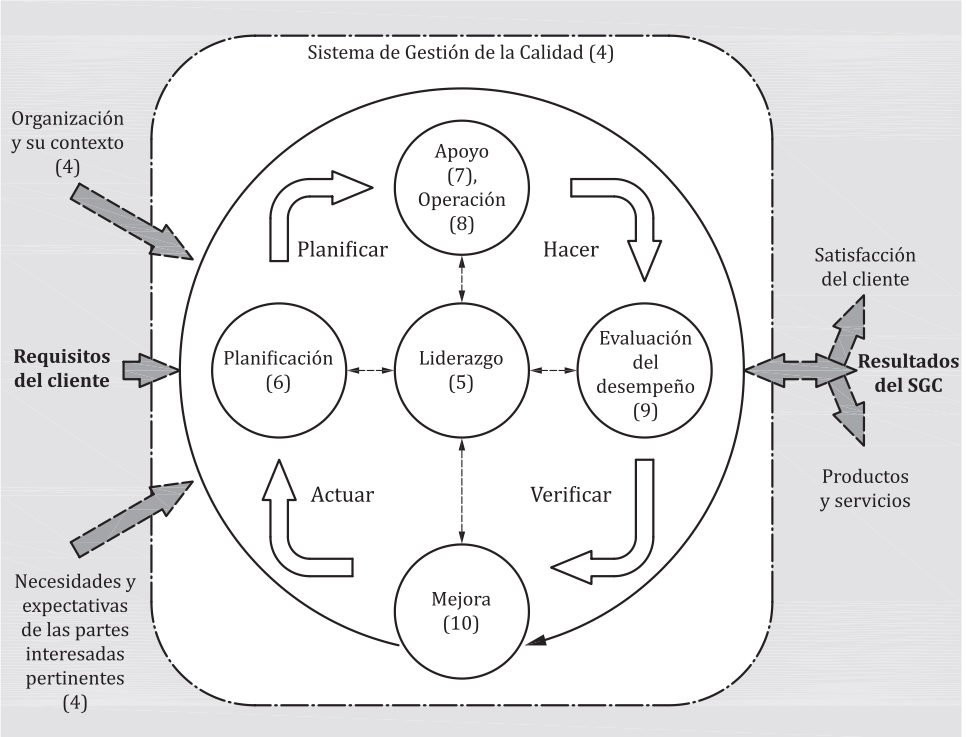
\includegraphics[width=\linewidth]{figura1.png}
	
				\par \noindent
					El ciclo PHVA puede describirse brevemente como sigue:
					\begin{itemize}
						\item Planificar: establecer los objetivos del sistema y sus procesos, y los recursos necesarios para
						generar y proporcionar resultados de acuerdo con los requisitos del cliente y las políticas de la
						organización, e identificar y abordar los riesgos y las oportunidades;
						
						\item Hacer: implementar lo planificado;
						
						\item Verificar: realizar el seguimiento y (cuando sea aplicable) la medición de los procesos y los productos
						y servicios resultantes respecto a las políticas, los objetivos, los requisitos y las actividades
						planificadas, e informar sobre los resultados;
						
						\item Actuar: tomar acciones para mejorar el desempeño, cuando sea necesario.
					\end{itemize}
				
				\newpage
				\thispagestyle{plain}
				
			\paragraph{Pensamiento basado en riesgos}\mbox{}
				
				El pensamiento basado en riesgos es esencial para lograr un sistema de gestión de la calidad eficaz. El concepto de pensamiento basado en riesgos ha estado implícito en ediciones anteriores de esta Norma Internacional, incluyendo, por ejemplo, llevar a cabo acciones preventivas para eliminar no conformidades potenciales, analizar cualquier no conformidad que ocurra, y tomar acciones que sean apropiadas para los efectos de la no conformidad para prevenir su recurrencia.
				
				\par \noindent
					Para ser conforme con los requisitos de esta Norma Internacional, una organización necesita planificar
					e implementar acciones para abordar los riesgos y las oportunidades. Abordar tanto los riesgos como
					las oportunidades establece una base para aumentar la eficacia del sistema de gestión de la calidad,
					alcanzar mejores resultados y prevenir los efectos negativos.
				
				\par \noindent
					Las oportunidades pueden surgir como resultado de una situación favorable para lograr un resultado
					previsto, por ejemplo, un conjunto de circunstancias que permita a la organización atraer clientes,
					desarrollar nuevos productos y servicios, reducir los residuos o mejorar la productividad. Las acciones
					para abordar las oportunidades también pueden incluir la consideración de los riesgos asociados. El
					riesgo es el efecto de la incertidumbre y dicha incertidumbre puede tener efectos positivos o negativos. Una desviación positiva que surge de un riesgo puede proporcionar una oportunidad, pero no todos los efectos positivos del riesgo tienen como resultado oportunidades.
					
		\subsection{ISO 17025:2005}
				
				

			
			
				
				